\documentclass[a4paper,11pt]{article}
\input{/home/tof/Documents/Cozy/latex-include/preambule_lua.tex}
\newcommand{\showprof}{show them}  % comment this line if you don't want to see todo environment
\fancyhead[L]{Diviser pour régner - correction exercices}
\newdate{madate}{10}{09}{2020}
\fancyhead[R]{Terminale - NSI} %\today
\fancyfoot[L]{~\\Christophe Viroulaud}
\fancyfoot[C]{\textbf{Page \thepage}}
\fancyfoot[R]{\includegraphics[width=2cm,align=t]{/home/tof/Documents/Cozy/latex-include/cc.png}}

\begin{document}
\begin{Form}
\begin{exo}
\begin{enumerate}
\item impératif
\lstinputlisting[firstline=29,lastline=43]{"scripts/dichotomie.py"}
\item récursif
\lstinputlisting[firstline=10,lastline=27]{"scripts/dichotomie.py"}
\item liste
\lstinputlisting[firstline=45,lastline=45]{"scripts/dichotomie.py"}
\item test
\lstinputlisting[firstline=46,lastline=49]{"scripts/dichotomie.py"}
\item L'algorithme de dichotomie est de complexité $O(log_2(n))$.
\end{enumerate}
\end{exo}
\begin{exo}
\lstinputlisting[firstline=9,lastline=21]{"scripts/tri_rapide.py"}
Ce tri n'est pas stable.
\end{exo}
\begin{exo}
\begin{figure}[!h]
\centering
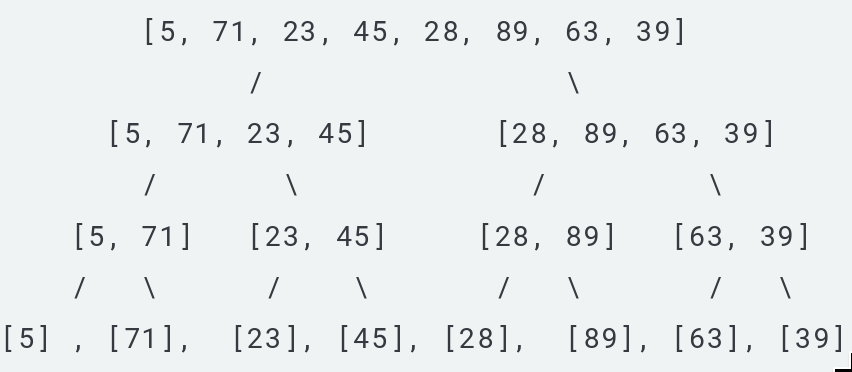
\includegraphics[width=10cm]{ressources/separation.png}
\captionof{figure}{Séparation}
\label{separation}
\end{figure}
\begin{figure}[!h]
\centering
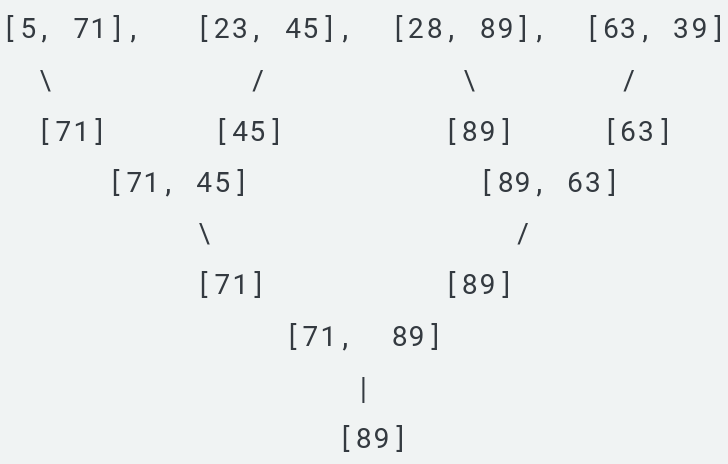
\includegraphics[width=10cm]{ressources/combinaison.png}
\captionof{figure}{Recombinaison}
\label{combinaison}
\end{figure}
\\Cette fonction renvoie le maximum de la liste.
\end{exo}
\end{Form}
\end{document}